\documentclass[12pt]{article}
\usepackage[scaled]{helvet}
\renewcommand\familydefault{\sfdefault} 
\usepackage[T1]{fontenc}

\usepackage[english]{babel}
\usepackage[utf8]{inputenc}
\usepackage{amsmath}
\usepackage{bm}
\usepackage{parskip}
\usepackage{hyperref}
\usepackage{graphicx}
\usepackage{listings}
\usepackage{xcolor}

\definecolor{Brown}{cmyk}{0,0.81,1,0.60}
\definecolor{OliveGreen}{cmyk}{0.64,0,0.95,0.40}
\definecolor{CadetBlue}{cmyk}{0.62,0.57,0.23,0}
\definecolor{lightlightgray}{gray}{0.9}

\lstset { %
    language=C++,
    %backgroundcolor=\color{black!5}, % set backgroundcolor
    %basicstyle=\footnotesize,% basic font setting
	basicstyle=\ttfamily,                   % Code font, Examples: \footnotesize, \ttfamily
	keywordstyle=\color{OliveGreen},        % Keywords font ('*' = uppercase)
	commentstyle=\color{gray},              % Comments font
	backgroundcolor=\color{lightlightgray},
	tabsize=4,
	frame=single,
}

\title{\textbf{Practical 5: Mass-Spring Systems, part 2 }}
\author{Babis Koniaris}
\date{}

\begin{document}
\maketitle

\begin{center}
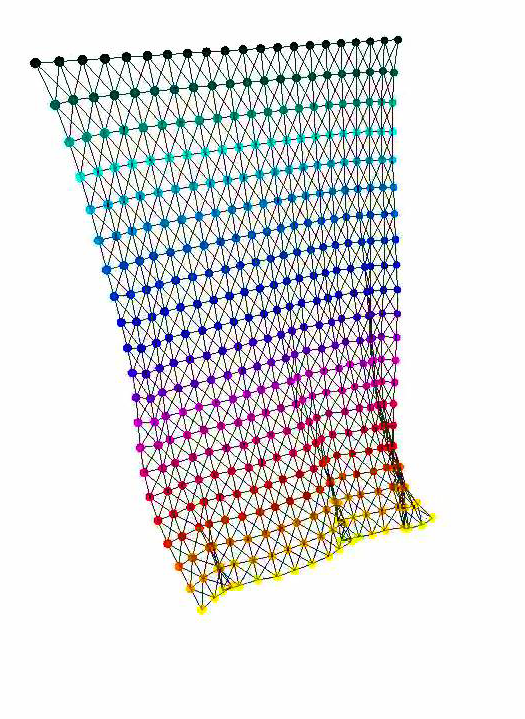
\includegraphics[width=0.7\textwidth,height=\textheight,keepaspectratio]{p5-teaser.png}
\end{center}
\pagebreak

\section*{Introduction}

The goals of this practical are to:

\begin{itemize}
\item Improve your practical understanding of mass-spring systems
\item Implement 1D and 2D mass-spring system simulations
\end{itemize}

You will continue working on and evolving the same project: ``03\_constraints\_framework''.

\section*{Tasks}

\subsection*{Chain of particles connected by springs}

This is identical to task 3 from last week, and is only included here to keep the assessed tasks together.

\subsection*{Chain of particles connected by damped springs}

\textbf{Task 2: Simulate a chain of 10 particles connected to each other by a damped spring}

The system is assumed to be under the influence of gravity. The two extremities of the chain should be fixed at the same height. It should look approximately like mass\_spring\_systems\_1d\_b.exe.

\subsection*{Chain of particles connected by damped springs, plus collision with plane}

\textbf{Task 3: Same as task 2, but particles collide with the ground plane}

It should look approximately like mass\_spring\_systems\_1d\_c.exe.

\subsection*{Cloth simulation 1}

\textbf{Task 4: Simulate a square piece of cloth whose 4 corners are fixed to points located at the same height}

\begin{itemize}
\item Use a 10$\times$10 particle array. You can use:
	\begin{itemize}
	\item C-style arrays, e.g. Particle particles[10][10]
	\item std::array<Particle, 100>
	\item std::vector<Particle>
	\end{itemize}
\item Include collision detection with plane, as per previous task
\item The cloth should be aligned with the XZ axis, like a trampoline. 
\item It should look approximately like mass\_spring\_systems\_2d\_a.exe.
\item You should use, at a minimum, structural constraints, but you might find that the simulation is better with shear constraints and bending constraints.
\end{itemize}

\subsection*{Cloth simulation 2}

\textbf{Task 5: Simulate a square piece of cloth where two adjacent corners are attached to fixed points in space located at the same height. Add a variable (horizontal) wind effect or moving (horizonta ) blow-dryer to your scene}

The cloth structure will be identical to the one created in the previous task, but with different fixed particles. The real challenge that you need to address to get full marks for this practical is the implementation of a force field (wind or blow dryer) that applies to the cloth geometry, not to the particles themselves. Without wind, it should look approximately like mass\_spring\_systems\_2d\_b.exe.

\section*{Deliverables}

This week's work (and a bit from last week) is assessed, so you need to submit evidence of completed tasks to gain credits.

\subsection*{Marking scheme}

Here's a summary of what you need to deliver, and the associated marks:

\begin{itemize}
\item \textbf{Chain of particles connected by springs (Task 1): 4 marks}
\item \textbf{Chain of particles connected by damped springs (Task 2): 4 marks} 
\item \textbf{Chain of particles connected by springs, plus collision with plane (Task 3): 4 marks}
\item \textbf{Cloth simulation 1 (Task 4): 4 marks}
\item \textbf{Cloth simulation 2 (Task 5): 4 marks} 
\end{itemize}

\subsection*{Submission details}

You must submit your work using the relevant Moodle assignment by the deadline specified on Moodle. Please submit, in a zip file:

\begin{itemize}
\item Your source code (/path-to-repository/code/03\_constraints\_framework)
\item A working executable (/path-to-repository/code/build/bin/03\_constraints\_framework)
\item Instructions of how to use the program (key mappings, etc) as a text file
\end{itemize}

Marks will only be granted when a working application is demonstrated in the lab or via screen-sharing video.

\end{document}